\documentclass{report}

\usepackage{physics}
\usepackage{graphicx}
\usepackage{hyperref}

\usepackage{listings}
\usepackage{color}

\definecolor{red}{rgb}{1,0,0}
\definecolor{dkgreen}{rgb}{0,0.6,0}
\definecolor{gray}{rgb}{0.5,0.5,0.5}
\definecolor{mauve}{rgb}{0.58,0,0.82}

\renewcommand{\thesection}{\arabic{section}}
\setcounter{secnumdepth}{3}
\setcounter{tocdepth}{3}

\hypersetup{
    colorlinks=true,
    linkcolor=blue,
    filecolor=magenta,      
    urlcolor=blue,
}

\lstset{
    frame=tb,
    language=Python,
    aboveskip=3mm,
    belowskip=3mm,
    showstringspaces=false,
    columns=flexible,
    basicstyle={\small\ttfamily},
    numbers=none,
    numberstyle=\tiny\color{gray},
    keywordstyle=\color{blue},
    commentstyle=\color{dkgreen},
    stringstyle=\color{mauve},
    breaklines=true,
    breakatwhitespace=true,
    tabsize=3
}

\title{COVID-19 Data Analysis}

\author{Rishav Bhagat}

\graphicspath{{../res/imgs/}}

\begin{document}
    \maketitle
    \tableofcontents
    \newpage
    \section{Dataset}
        I used the dataset that was collected and used by John Hopkins University for 
        \href{https://www.arcgis.com/apps/opsdashboard/index.html#/bda7594740fd40299423467b48e9ecf6}{this project}. 
        This dataset was collected from many international health organizations and all compiled into onto github repository. 
        It contains information on daily reports (including new cases, deaths, and recoveries), and global trends. 
        \newline \indent
        Here is the link to the datasets I used: 
        \newline\indent\indent \href{https://github.com/CSSEGISandData/COVID-19}{https://github.com/CSSEGISandData/COVID-19}
        \subsection{Downloading the Data}
            I created a batch script to download all this data using git, delete files that are not needed for my analysis, and move the files into more convienient locations.
            \begin{lstlisting}
                @echo off
                rmdir data /s /q
                git clone https://github.com/CSSEGISandData/COVID-19.git
                rename COVID-19 data
                cd data
                rmdir .git /s /q
                rmdir archived_data /s /q
                rmdir who_covid_19_situation_reports /s /q
                del README.md
                mv csse_covid_19_data/* .
                rmdir csse_covid_19_data /s /q
                cd ..
                git add data
                git commit -m "updated data from John Hopkins github repo"
                git push
            \end{lstlisting}
        \subsection{Initial Glance}
            First, I plotted the global coronavirus data (cases vs days) in a similar fashion to the way it was plotting on the John Hopkins project. This is to reveal any obvious trends.
            \begin{center}
                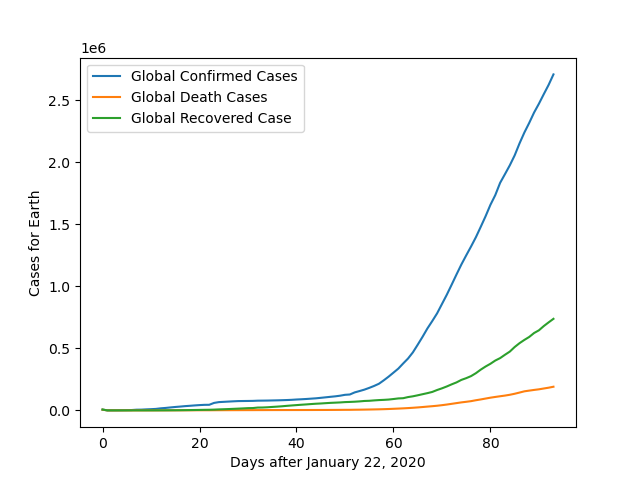
\includegraphics[width=10cm]{plots/global/cases.png}
            \end{center}
            At a first glance, this looks like exponential growth, so I then plotting a logarithmic graph with a line of best-fit.
            \begin{center}
                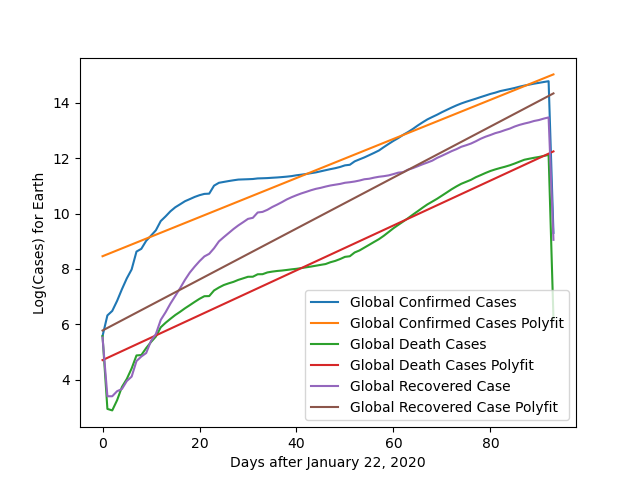
\includegraphics[width=10cm]{plots/global/log(cases).png}
            \end{center}
            A linear relationship in the logarithmic graph corresponds to an exponential relationship in the original graph. As we can see, the logarithmic graph is approximately linear, which confirms that so far, the coronavirus is exponentially growing. But we also see that the curve is beginning to flatten out, corresponding to the true logistic growth of the original graph. The beginning of all logarithmic graphs appear to be exponential, which explains why it apears as it does. 
            \newline
            \indent Now, we know that logistic growth will eventually level out, and it is in our interest to see when and where it will do this globally. We can do this by tracking the growth rate of the graph, as we shall see in the next section. 
    \section{Data Analysis and Implications}
        \indent First let's define some variables:
        \begin{itemize}
            \item Let us refer to the region we are talking about as $X$. For now $X$ refers to the entire globe.
            \item Let $N^X$ be the final number of people who have COVID-19 within $X$. I may sometimes just use $N$, which will refer to the region in question at the time.
            \item Let $N^X_i$ be the current number of people who have COVID-19 within $X$ on the $i$-th day after January 22nd (which is when John Hopkins began collecting data).
            \item Let $\Delta N^X_i = N^X_i - N^X_{i - 1}$ be the number of new cases on a given day, defined by $i$.
            \item In a similar way, define $D^X, D^X_i, \Delta D^X_i$ as the people who died due to COVID-19 in the respective time frames.
            \item In a similar way, define $R^X, R^X_i, \Delta R^X_i$ as the people who recovered from COVID-19 in the respective time frames.
        \end{itemize}
        While doing the analysis on the data, I will focus on the number of cases, but the number of deaths and recoveries also follow very similar patterns.
        \subsection{Growth Ratio}
        Another intrinsic value that can give us insight into the data is the growth ratio. Let's define this as
        \begin{equation}
            GR^X_i = \dfrac{N^X_i}{N^X_{i - 1}}
        \end{equation}
        For pure exponential growth the ratio should be a constant number throughout the entire domain, but since the ratio is decaying with time (as we see in the graph below), there is more evidence pointing to a more logistic approach. We see that the growth ratio is approaching one for both the cases and deaths, showing that eventually $N^X_i \rightarrow N^X$.
        \newline
        \indent Another interesting observation that is made apparant from this graph is the relationship between the deaths and cases. In other graphs this relationship is also evident, but here they are both plotted on the same scale so it is even more clear. The deaths are following a similar pattern as the cases, but they are slightly time-shifted (forward in time). This makes sense since we would expect a ratio of cases to become death in a certain time.
        \newline
        \indent We can also estimate the effectiveness of our treatment by checking if the death ratios start to become less that the cases ratios, but it is clear that this is not the cases currently, implying that we have not yet found a proper treatment.
        \newline
        \indent A further and more rigorous analysis of this graph and more detailed data could also give us insight to how long it takes the coronavirus to cause death on average.
        \begin{center}
            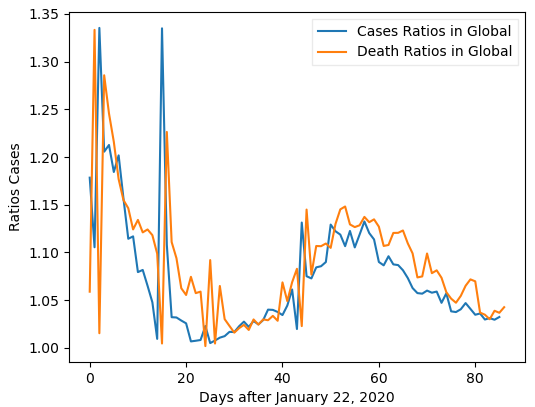
\includegraphics[width=10cm]{plots/global/growth_ratios.png}
        \end{center}
        \subsection{Growth Rate}
        Now we can define our growth rate as 
        \begin{equation}
            G^X_i = \dfrac{\Delta N^X_i}{\Delta N^X_{i - 1}}
        \end{equation}
        We are interested when this value crosses from $G > 1$ to $G < 1$, which corresponds to a point of infection. It is when the numbers of new cases each day begins to decrease rather than increase. Or in terms of calculus, when the second derivative becomes negative. The reason we do not just use the second derivative is that this data is noisy and approximating a high-order derivative would not work too well. Now plotting the growth rate:
        \begin{center}
            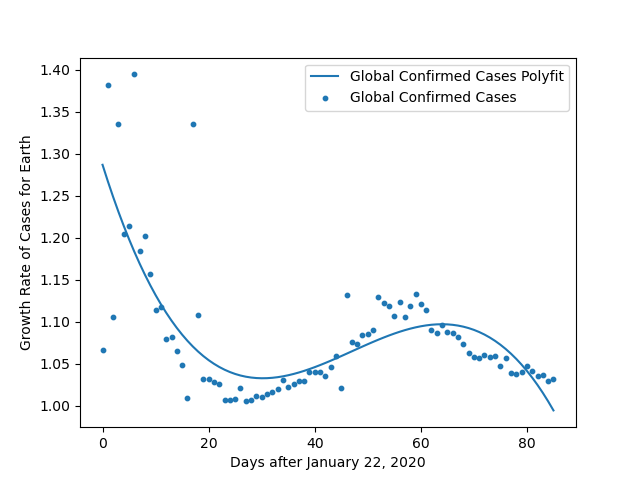
\includegraphics[width=10cm]{plots/global/growth_rate.png}
        \end{center}
        If the graph continues to follow the polyfit curve drawn, then we expect the inflection point to occur soon, but we do not know if it will go back up as it did at around $i = 25$. In fact, we can expect it to go up, which is evident by plotting the approximated derivative
        \footnote{
            When I refer to the derivative I am using the central difference approximation give by:
            $$f'(x) \approx \dfrac{f(x + h) - f(x - h)}{2h}$$
            with $h = 1$ since we have a discrete input space (each day).
            } of the growth function.
            \begin{center}
                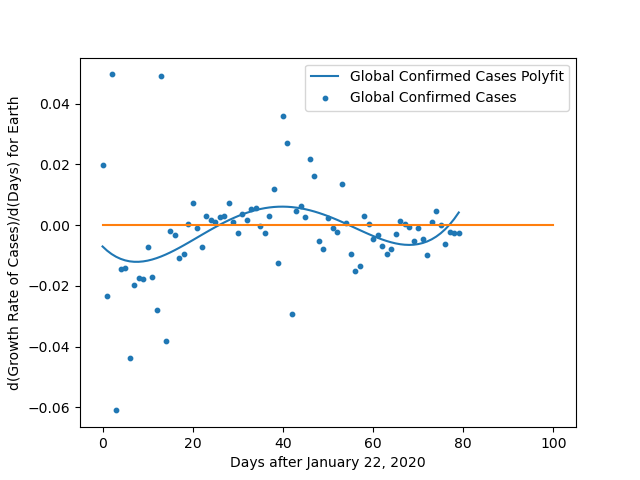
\includegraphics[width=10cm]{plots/global/growth_rate_derivative.png}
            \end{center} 
            The derivative of the growth rate at the current time ($i \approx 80$) is following the same pattern as at $i = 25$ and it has gone above the zero-line, implying that the growth rate will increase again.
            \newline
            \indent This is a dissapointing result since finding the true point of inflection will let us estimate where the number of cases will max out. If the point of inflection occurs at $i$, then it is reasonable to guess that the number of cases will max at $2 * N^X_i$ by the way logistic growth works.
            \subsubsection{Modelling with the Growth Rate}
            The curve generated by \lstinline{np.polyfit} fits the growth rate pretty well, so it may be possible to create a model based on the growth rate. To do so, we just have to follow the definitions of the growth rate and the solve for $N_i$:
            \begin{align*}
                G^X_i = \dfrac{\Delta N^X_i}{\Delta N^X_{i - 1}} = \dfrac{N^X_i - N^X_{i - 1}}{N^X_{i - 1} - N^X_{i - 2}} \\
                G^X_i(N^X_{i - 1} - N^X_{i - 2}) = N^X_i - N^X_{i - 1}
            \end{align*}
            and finally
            \begin{equation}
                N^X_i = N^X_{i - 1} + G^X_i(N^X_{i - 1} - N^X_{i - 2})
            \end{equation}
            But there are a lot of problems with a model like this. For one it is based on previous estimates, so any error in early estimates will propagate through to the later estimates, making the model extremely inaccurate for anything too far out of the domain of the data.
            \newline
            \indent Also, as we showed before, the growth rate will likely not follow the polyfit curve outside the domain of the data.
        \subsection{Derivative}
            The derivative (approximated) of $N^X_i$ with respect to $i$, or $\dfrac{dN^X_i}{di}$, is an important value to look at since it can also help us classify the type of model the spread of coronavirus is following. In an exponential model, we would see $\dfrac{dN^X_i}{di} \propto N^X_i$, while in a logistic model we would expect $\dfrac{dN^X_i}{di} \propto (1 - N^X_i / N^X)N^X_i$. Now plotting the derivative:
            \begin{center}
                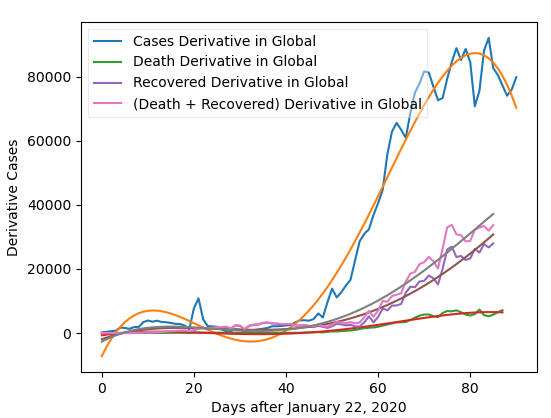
\includegraphics[width=10cm]{plots/global/derivative.png}
            \end{center}
            As expected the derivative is never negative since that would meann the number of cases are going down, which is impossible (since the number of cases is defined as the number of all cases recorded and does not decrement from recoveries).
            \newline
            \indent Putting this graph next to one of the number of cases, we can compare them to see proportionality and see what type of model the spread is following. I will do this with the Analysis Dashboard for Global Cases, which I talk about more in \hyperref[sec:country]{Section 2.5}
            \begin{center}
                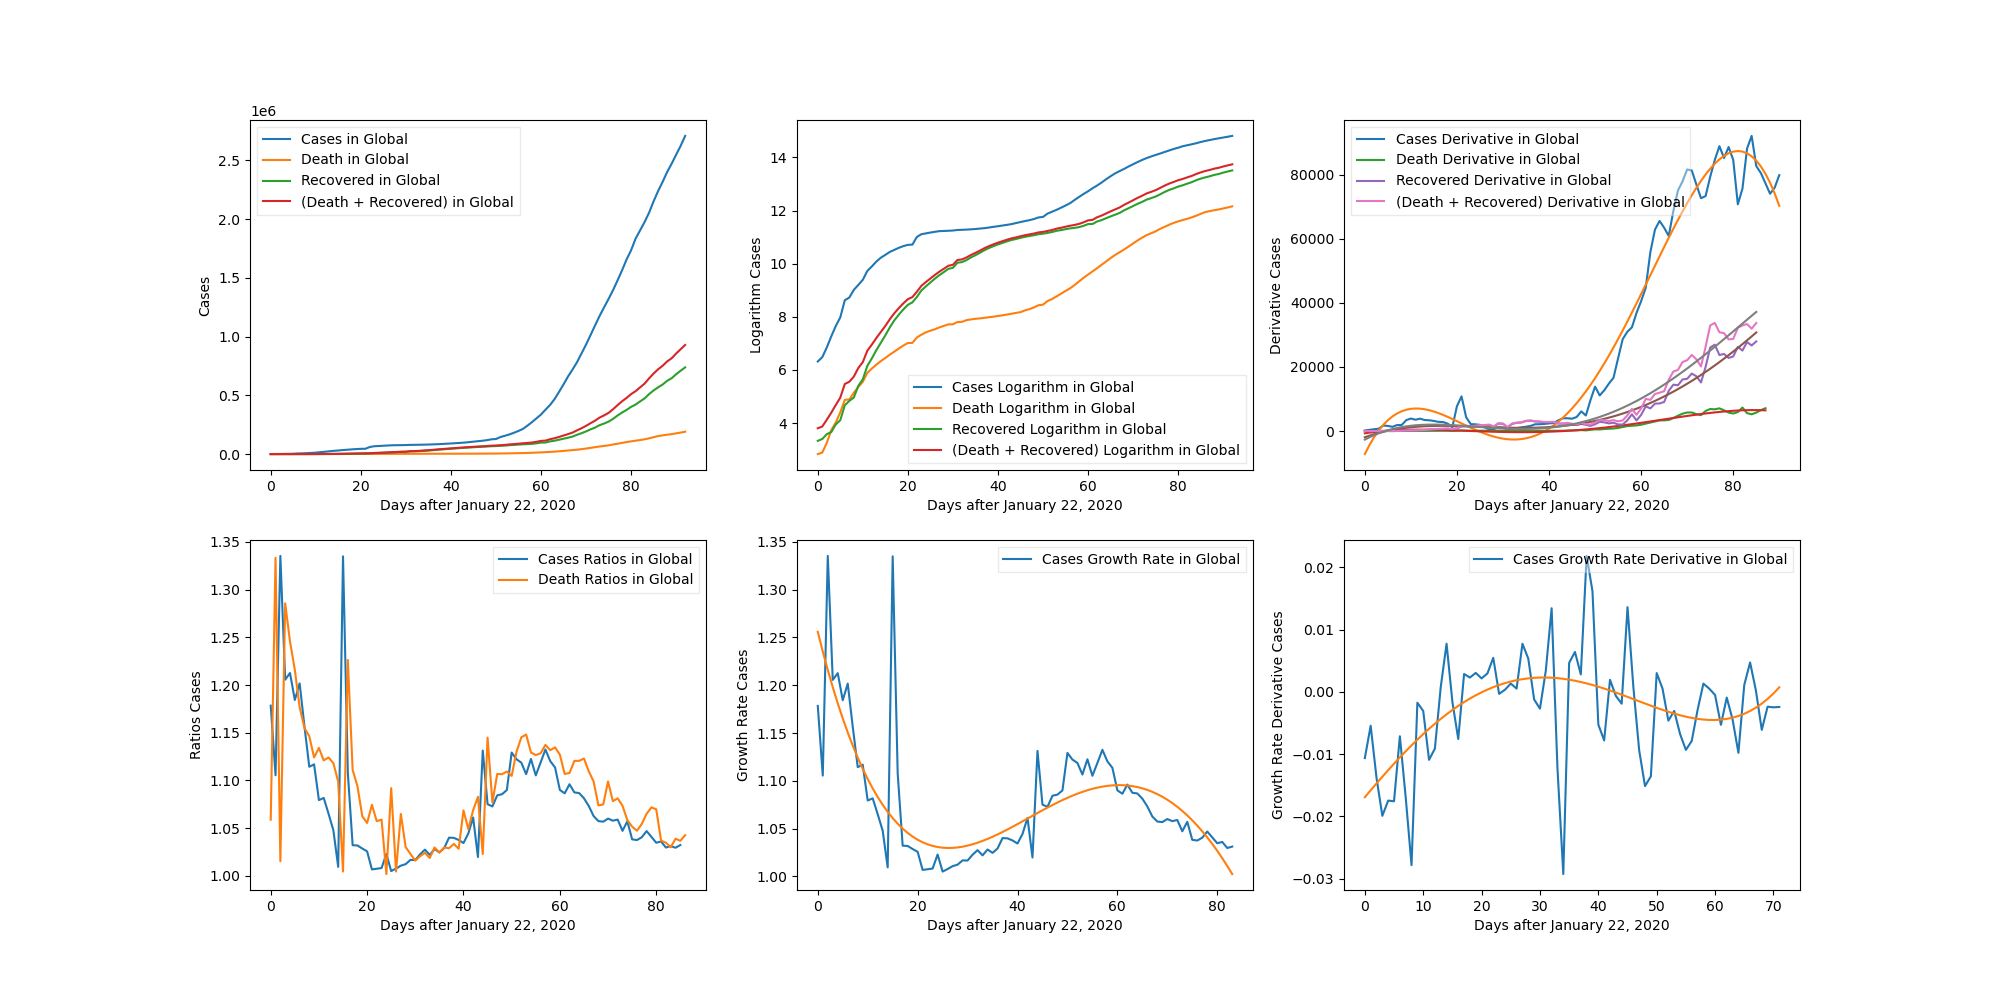
\includegraphics[width=\textwidth]{plots/global/analyze.png}
            \end{center}
            The derivative is initially approximately proportion to the number of cases, which is seen by looking at the first and third graphs. But then the derivative starts to level off as expected by logistic growth. The derivative is starting to decrease implying a critical point. Now if we assume that the graph will continue to fall in this manner we can expect the derivative to go back to 0 at around $i=120$, or about 4 months after January 22, which puts us at around the end of May. Once the derivative is back at zero there will be no new cases and the virus will have stopped spreading. But a crude prediction such as that one does not account for skew, since chances are that the graph will be right skewed, since that is how logistic graphs are. Accounting for this we can expect the curve to flatten out a bit later than the end of May. 
            \newline
            \indent Another option is that we can try to use an initial subset of the data to try to estimate the proportionality constant $c$ by
            \begin{equation}
                \dfrac{dN^X_i}{di} = c(1 - N^X_i/N^X)N^X_i
            \end{equation}
            where $(1 - N^X_i/N^X) \approx 1$ (in the initial subset), so $\dfrac{dN^X_i}{di} \approx cN^X_i$. After finding $c$, we can use the graph for the derivative to estimate $N^X$, assuming a perfectly logistic model. I will actually implement this in \hyperref[sec:auto]{Section 2.6}.
        \subsection{Fitting Polynomials to Subsets of the Data}
        \label{sec:polys}
            The numpy module has a \lstinline{polyfit} method that can take a bunch of data and fit a polynomial of a given degree to it. In theory, this can be used to create a model for the COVID-19 data, but there are many problems with this\footnote{I go further in depth into these problems in \hyperref[sec:problems]{Section 3.1}}. But we can still use a technique like this to gain insights into our data.
            \subsubsection{Finding the Best Degree for Polyfit}
                Just like any other model, we can measure how well the generated polynomial fits the data using some sort of loss function. I used mean squared error, defined by
                \begin{equation}
                    MSE(\vec{p}, (N^X_i)) = \dfrac{1}{N}\sum_{i=0}^{N - 1}(N_i^X - \vec{p} \cdot \vec{x}(i))^2
                \end{equation}
                for our polynomial model, where $\vec{p}$ is a vector containing the weights for our polynomial model, $N$ is the number of samples. The function $\vec{x}(i)$ returns a vector defined by
                \begin{equation}
                    x(i) = [i^m, i^{m - 1}, i^{m-2}, \dots, i^2, i, 1]
                \end{equation}
                where $m$ is the polynomial's degree. The vectors $\vec{p}$ and $\vec{x}(i)$ have length $m + 1$. Here $x$ acts as a feature transformer. 
                \newline\indent
                Now to find the smallest $m$ that has a good fit to our data, I track the ratio between the impovement since $m - 1$ and the original $MSE$ with $m = 1$ and increment $m$ until it is less than a theshold $\epsilon$. Essentially I find the smallest $m$, where
                \begin{equation}
                    \dfrac{MSE(\vec{p_m}, (N_i^X)) - MSE(\vec{p_{m - 1}}, (N_i^X))}{MSE(\vec{p_1}, (N_i^X))} < \epsilon
                \end{equation}
                where the $MSE$ for $m = 1$ is used as a scaling factor. After this we know that after $m - 1$ there is not going to be much improvement, so we do our polyfits on $m - 1$.
            \subsubsection{Correlations Between the Best Degree and Subsets of the Data}
                From now on, I will refer to $m$ as the best degree to use \lstinline{np.polyfit} with. I will use python subindexing, which is defined like this: If
                $$x = [1,2,3,4,5]$$
                then
                $$x[0:2] = [1,2]$$
                And it is [inclusive, exclusive]. Now define, $m(j) = \text{findBestDegree}((N_i^X)[0:j])$. Incrementing up $j$ and calculating $m(j)$, we are essentially finding a best fit polynomial of optimal degree for more and more of the data. Here is some of the polyfits for some subsets (incrementing by 10):
                \begin{center}
                    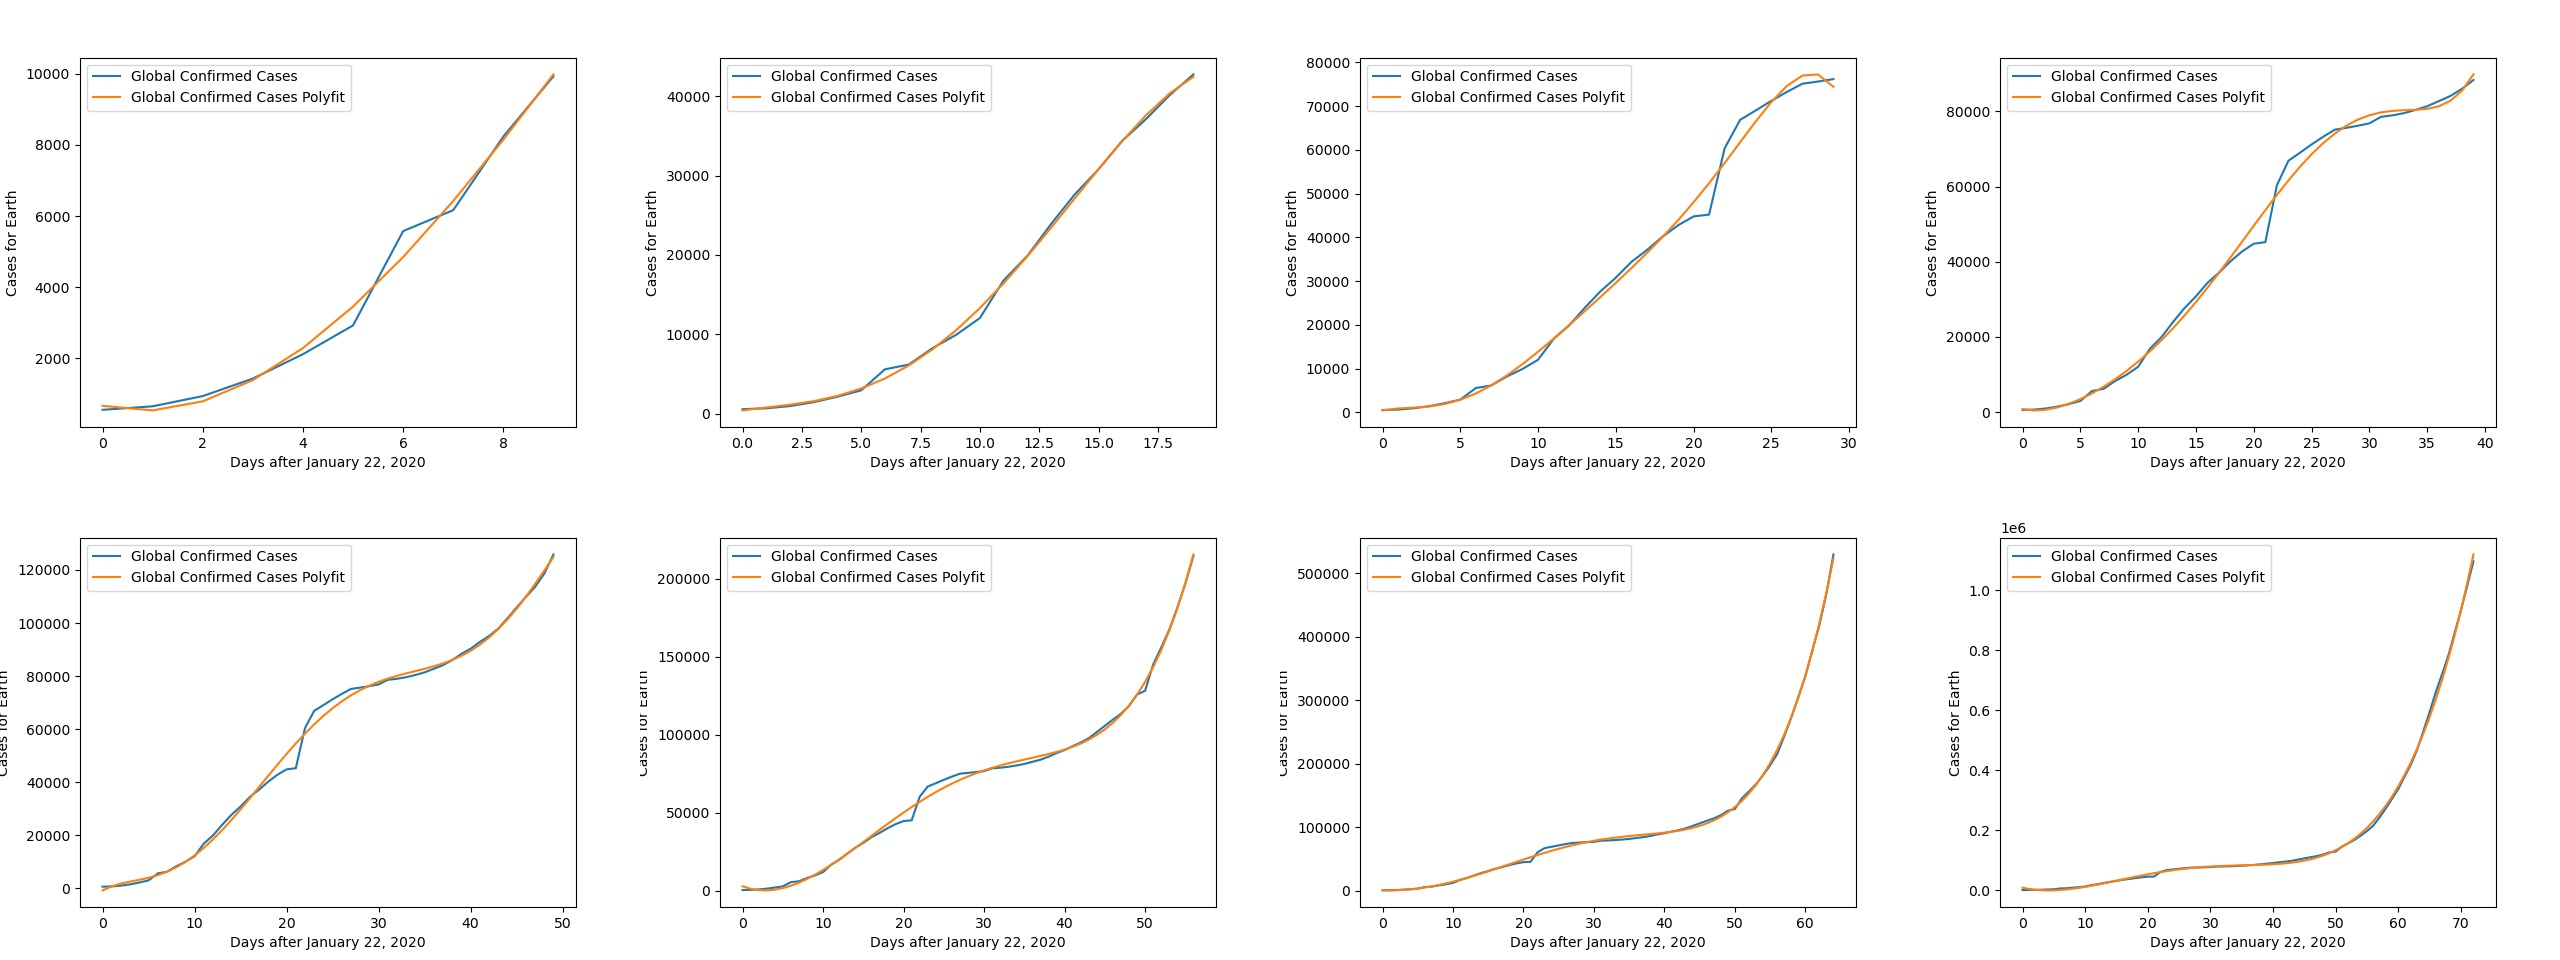
\includegraphics[width=\textwidth]{plots/global/fit-merged.png}
                \end{center}
                Now, there are two main factors in play as we increase $j$: there is more data to model, and the rate of change keeps increasing more as we get further in $(N_i^X)$, requiring a higher polynomial degree to model. Both of these require a higher degree to model as $j$ increases. 
                \begin{center}
                    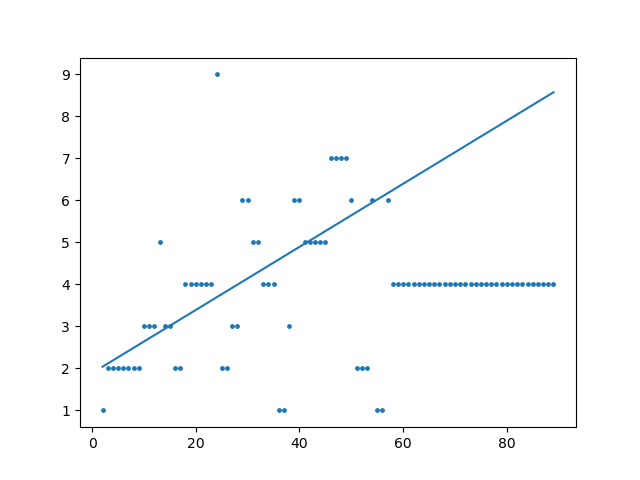
\includegraphics[width=10cm]{plots/global/degree_vs_subset.png}
                \end{center}
                In this plot the linear regression line is drawn based on the only the $j < 50$. And the graph exihibits the predicted pattern while $j < 50$, increasing $m$ with $j$, but after around $j = 55$, the $m$ stays constant at 4. Cross-referencing this with our previous finding that there is a point of inflection around that point (since $dG^X_i/di = 0$), I am guessing that the rate of change of the function slowed down enough for a polynomial of order $m = 4$ to model the graph.
                \newline\indent
                Another interesting thing to see is that the points on the graph are clustered, which makes sense since adding one point will likely not change $m$ by at least one everytime, and the output space is discrete, causing clusters to from. 
        \subsection{Country Analysis}
        \label{sec:country}
            To do an analysis of the countries, I will be using a "dashboard" with a bunch of graphs that each convey different information. Many of the graphs are talked about in previous sections talking about the global data. But now we will focus in on other regions (different values for $X$).
            \newline\indent
            Many of the observations I make will be in relation to the global dashboard since I have already done an in depth analysis of the global data. One of the difference that apply to all countries is that the graphs are scaled down from the global scale, but since we are analyzing trends, the amplitude does not matter too much. Another observation that applies to all the countries is that the data is noisier than on the global scale since there is less data.
            \begin{center}
                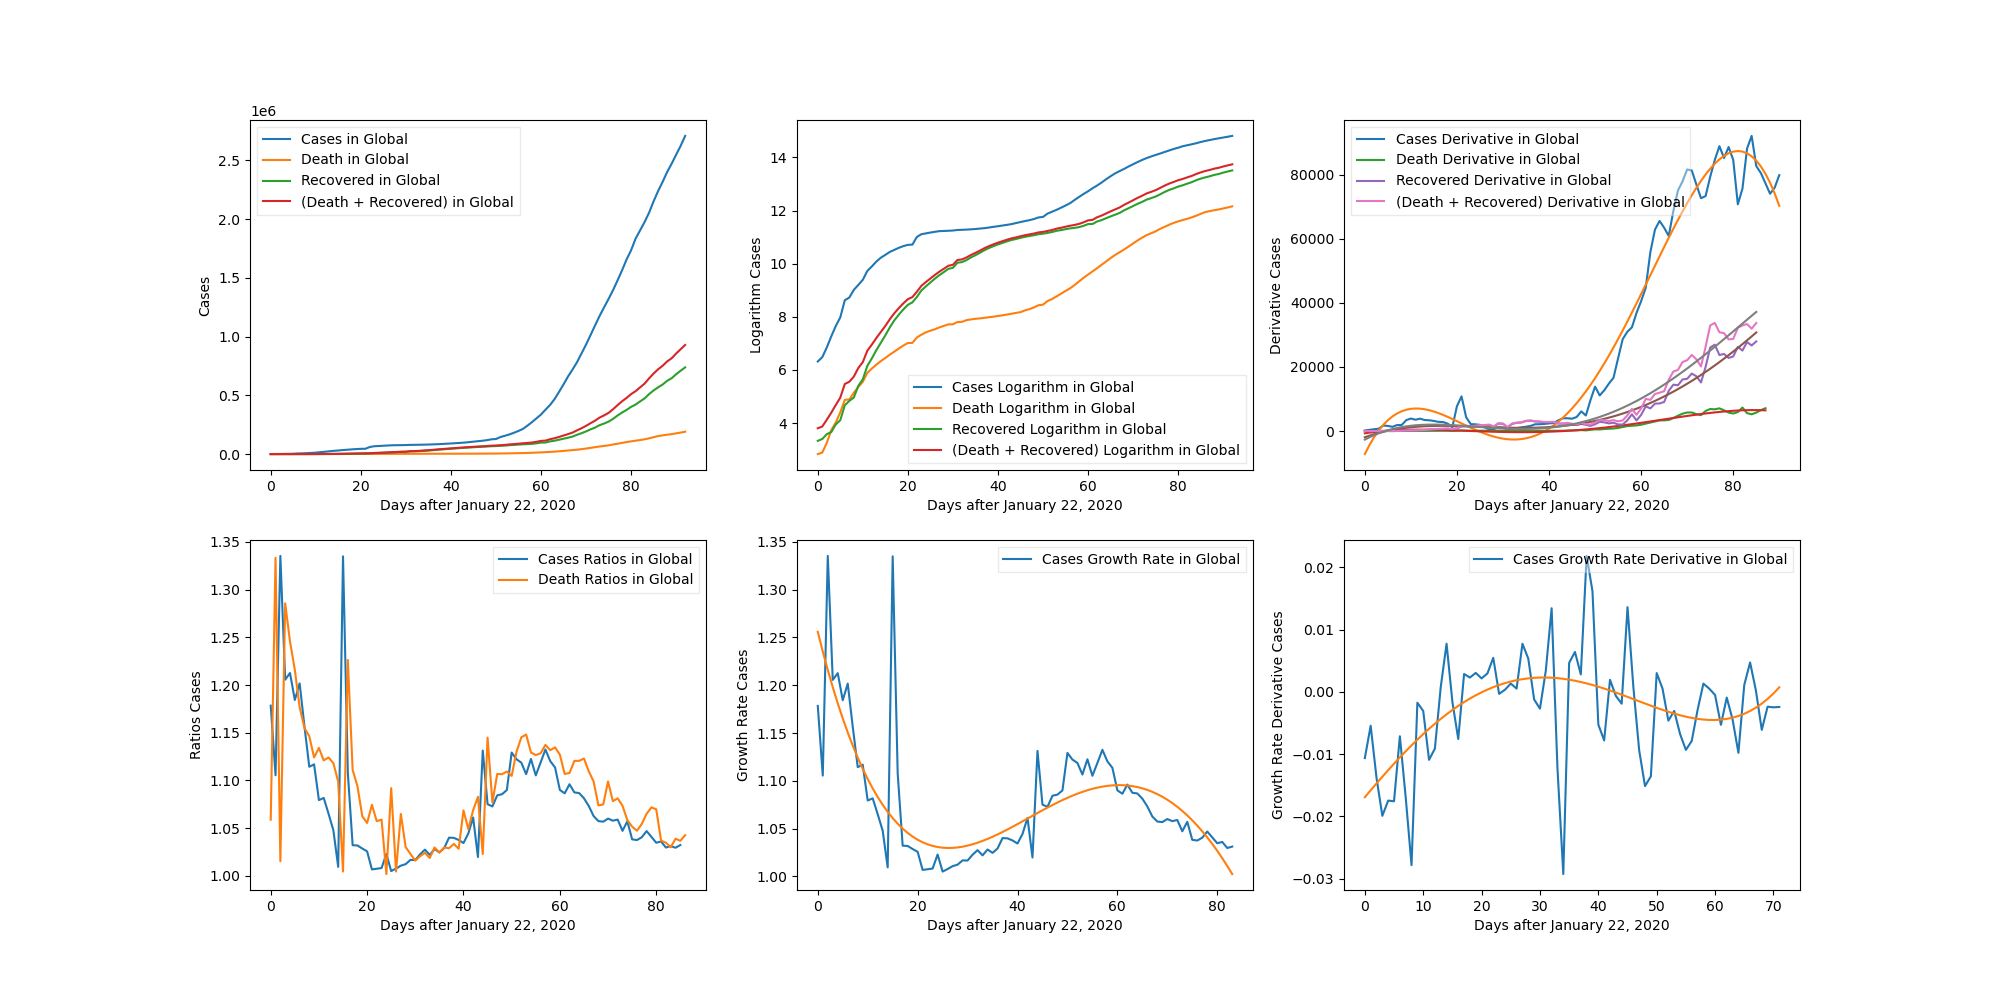
\includegraphics[width=\textwidth]{plots/global/analyze.png}
            \end{center}
            \subsubsection{United States}
                \begin{center}
                    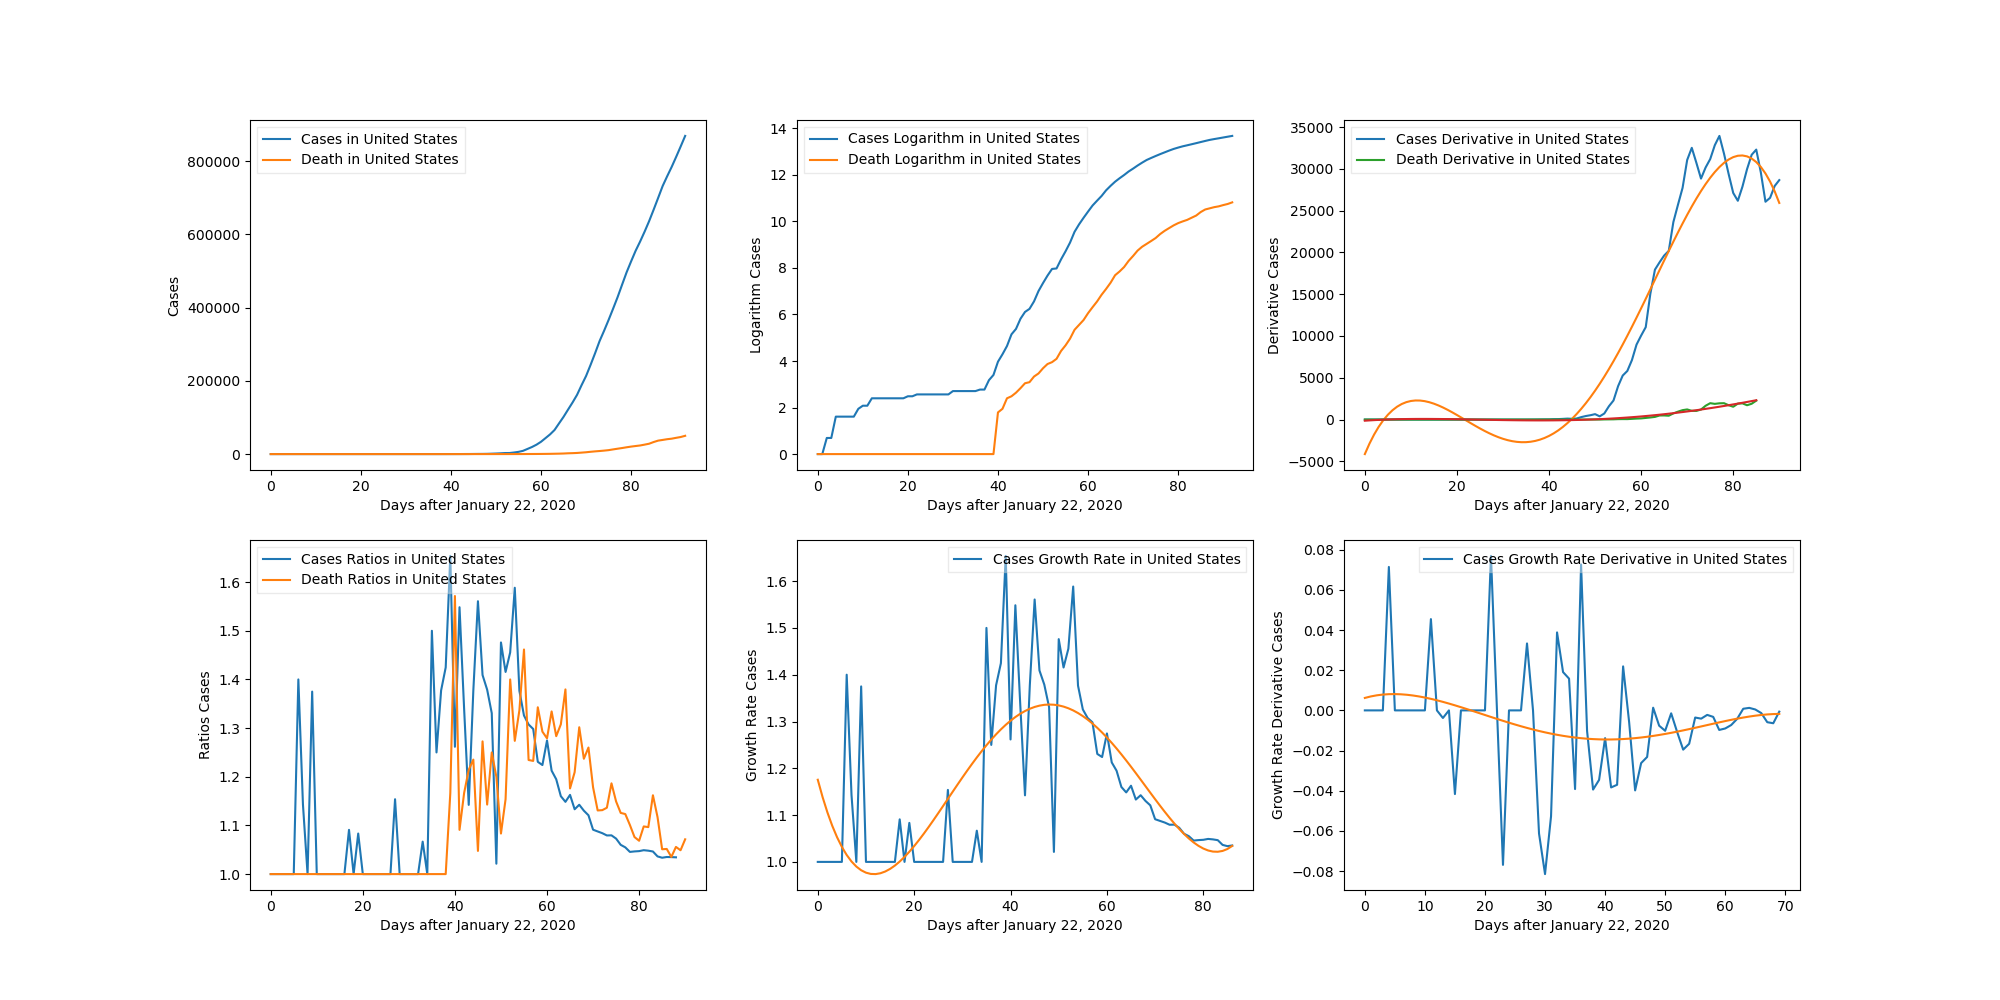
\includegraphics[width=\textwidth]{plots/united_states/analyze.png}
                \end{center}
                The trends that the United States graphs are following are similar to those of the global scale, except they are time shifted forward. This is a result of COVID-19 spreading to the United States later than it the average country. Up until around $i = 40$, the data is either near $0$ or does not follow any clear pattern. This is because the number of cases in the United States before that point was near 0. 
                \newline\indent
                Also, the logarithmic graph has only recently started to flatten out, meaning that the United States has been experiencing exponential growth of the coronavirus until recently. The is likely due to the late start in taking action against the virus. Another point is that the curves of the United States are flattening at around the same time as the global curves. So, since COVID-19 hit the United States pretty late, this shows that the United States is doing better than the globe as a whole.
            \subsubsection{China}
                \begin{center}
                    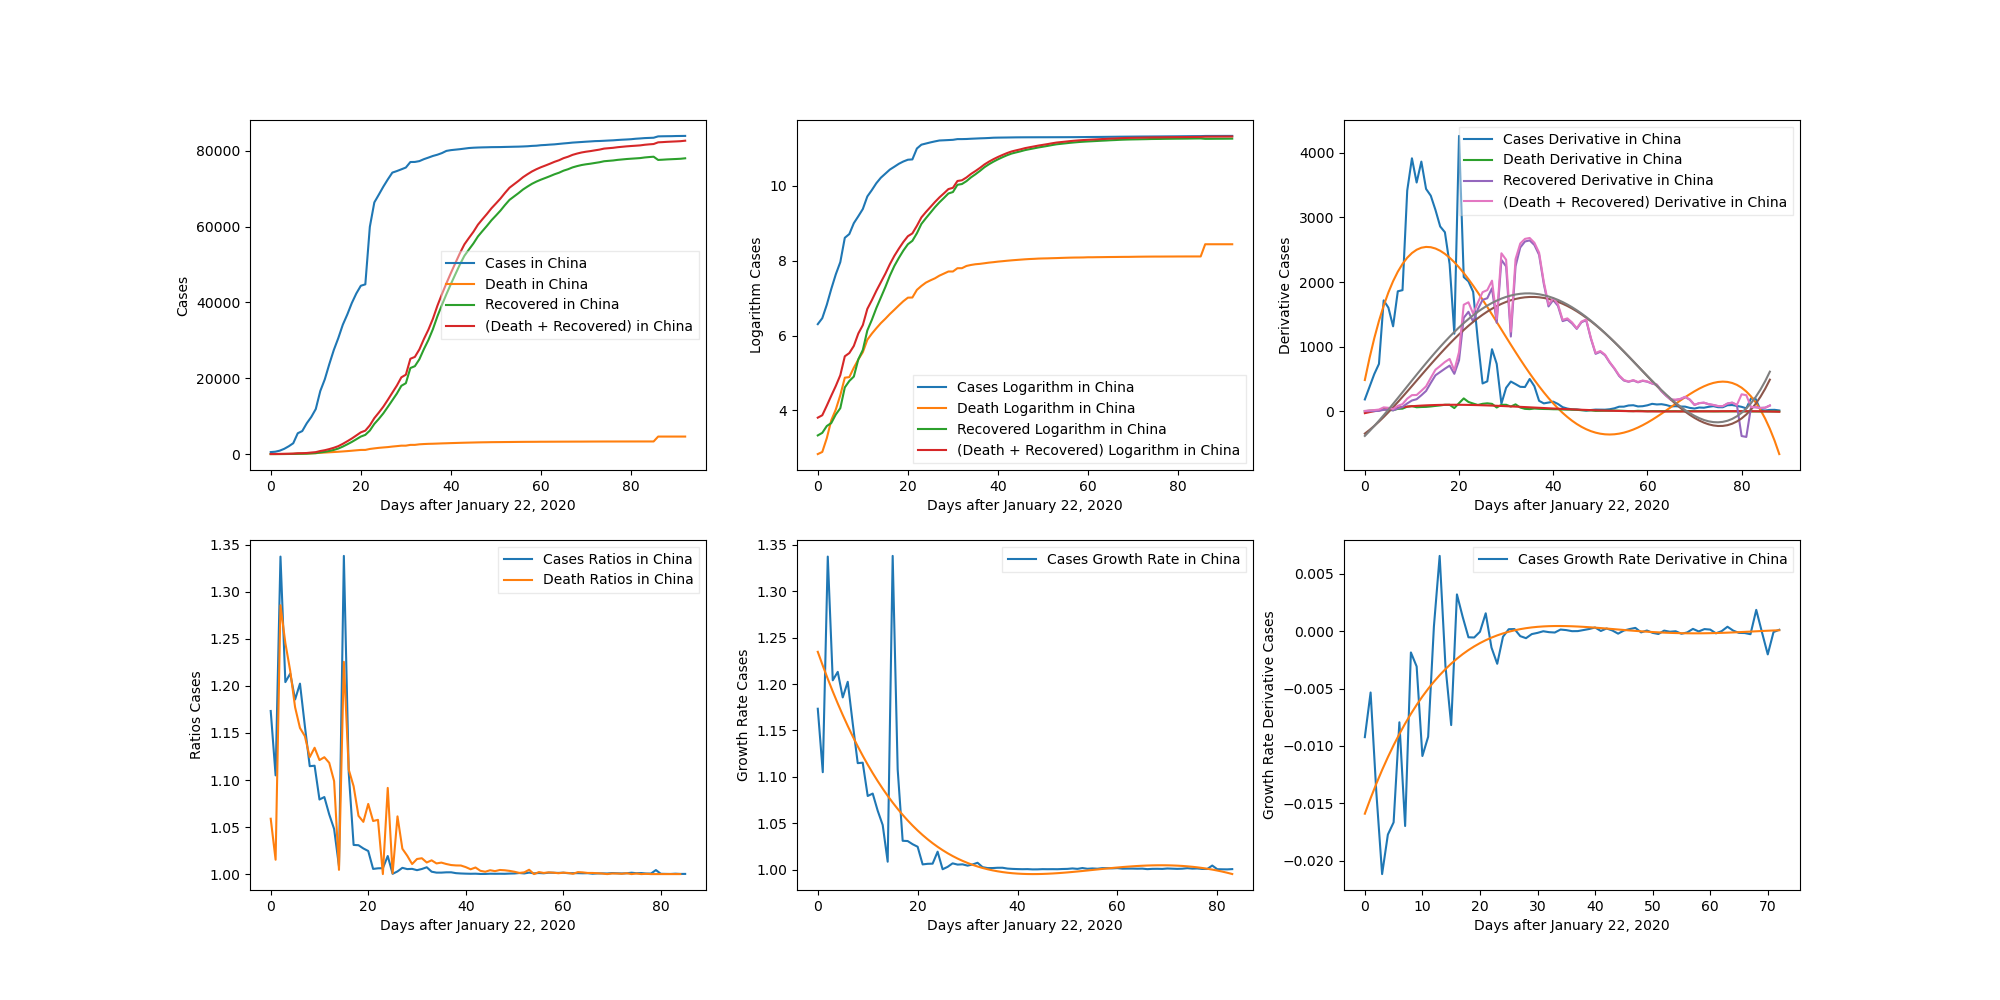
\includegraphics[width=\textwidth]{plots/china/analyze.png}
                \end{center}
                China's graphs are shifting backwards in time in relation to the global graphs, a result of the fact the virus started in China. Looking at the first graph we see that the difference between current cases and (death + recovered), or $N^{China}_i - (D^{China}_i + R^{China}_i)$, is approaching 0. That difference is the number of non-dealt with cases. China is the ideal model for logistic growth since we have data on the tail end of the growth. The growth ratio $GR^{China}_i$ and growth rate $G^{China}_i$ have both converged to 1, as seen by the graphs. Also, the graph of the cases follows a logistic growth curve. This flattening of the curve shows that China's strict policies are working in stopping the spread of the virus.
            \subsubsection{Italy}
                \begin{center}
                    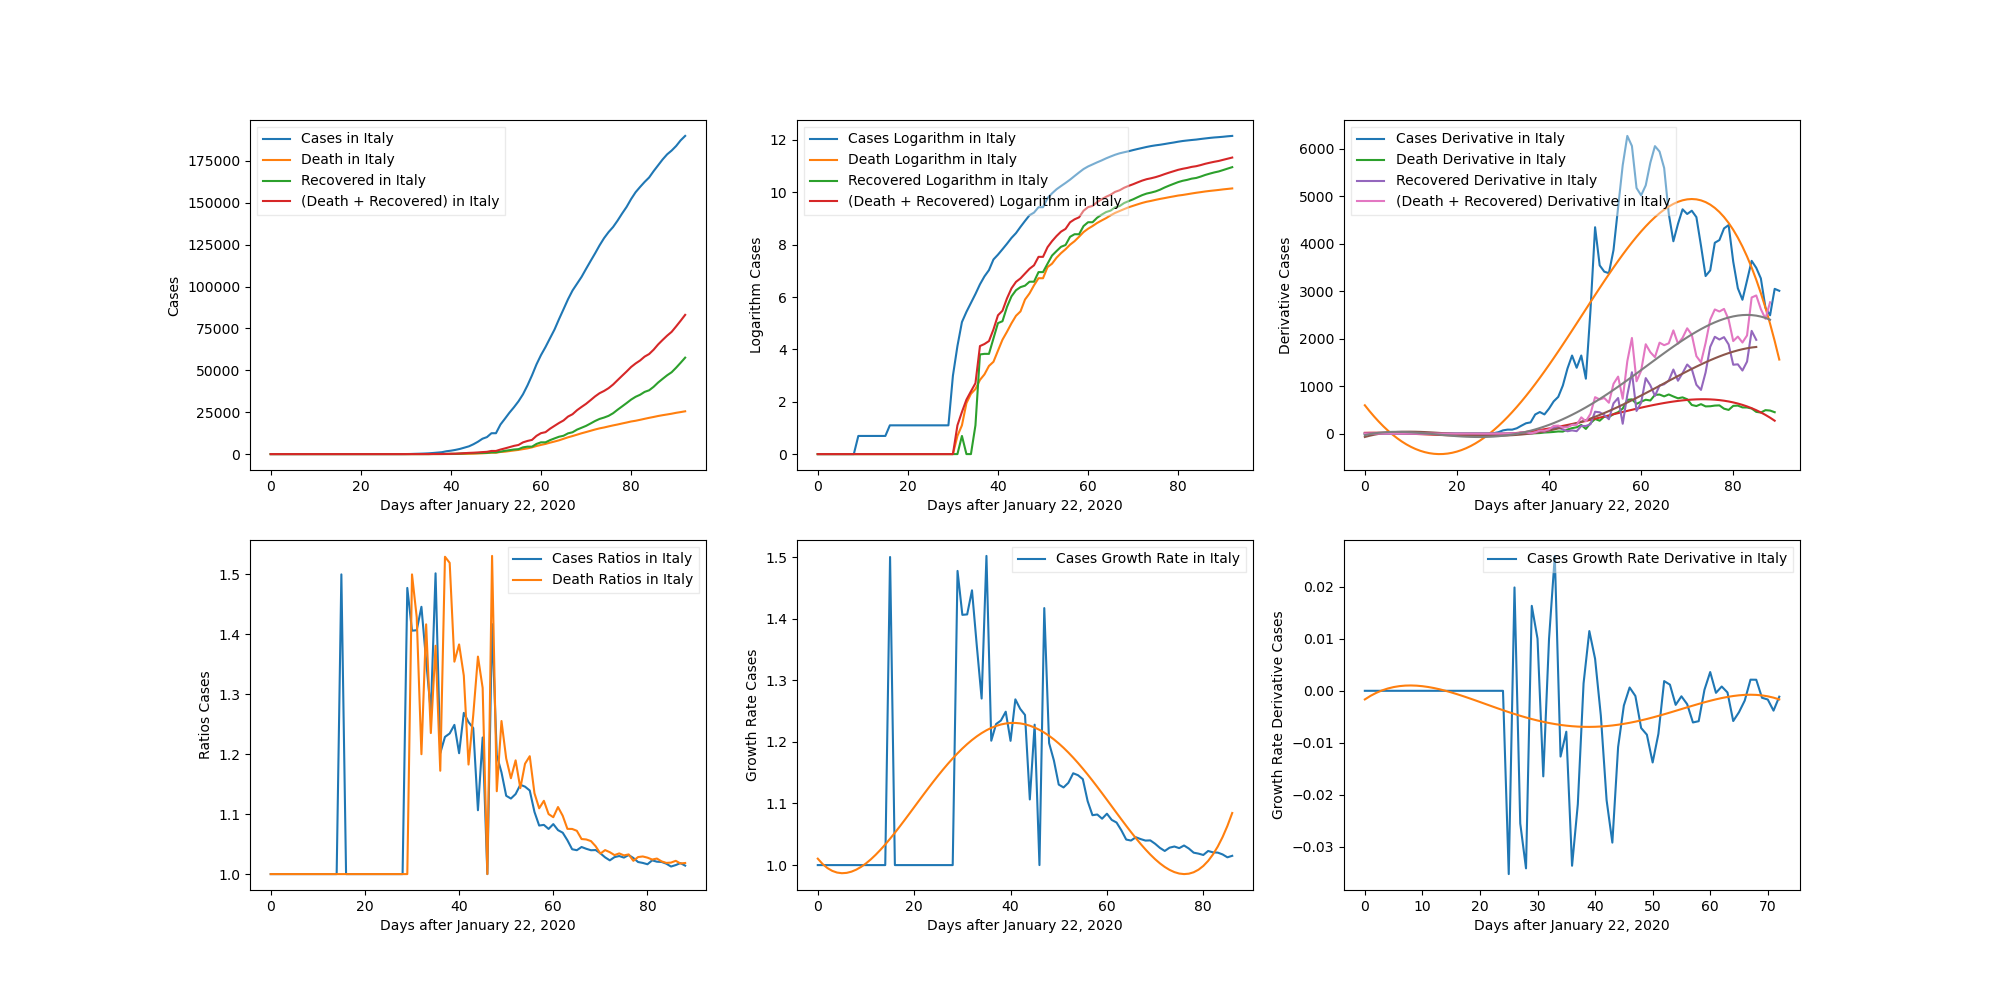
\includegraphics[width=\textwidth]{plots/italy/analyze.png}
                \end{center}
                Italy's graphs are time-shifted forward by about 10 less than the US graphs. Taking a look at the logarithmic graph, it is almost imediately flattening. This is unlike the previous couple countries, in which there was a longer time where the logarithmic graph was near linear. This correlated to Italy being well prepared for the virus and taking proper action against it.
            \subsubsection{Spain}
                \begin{center}
                    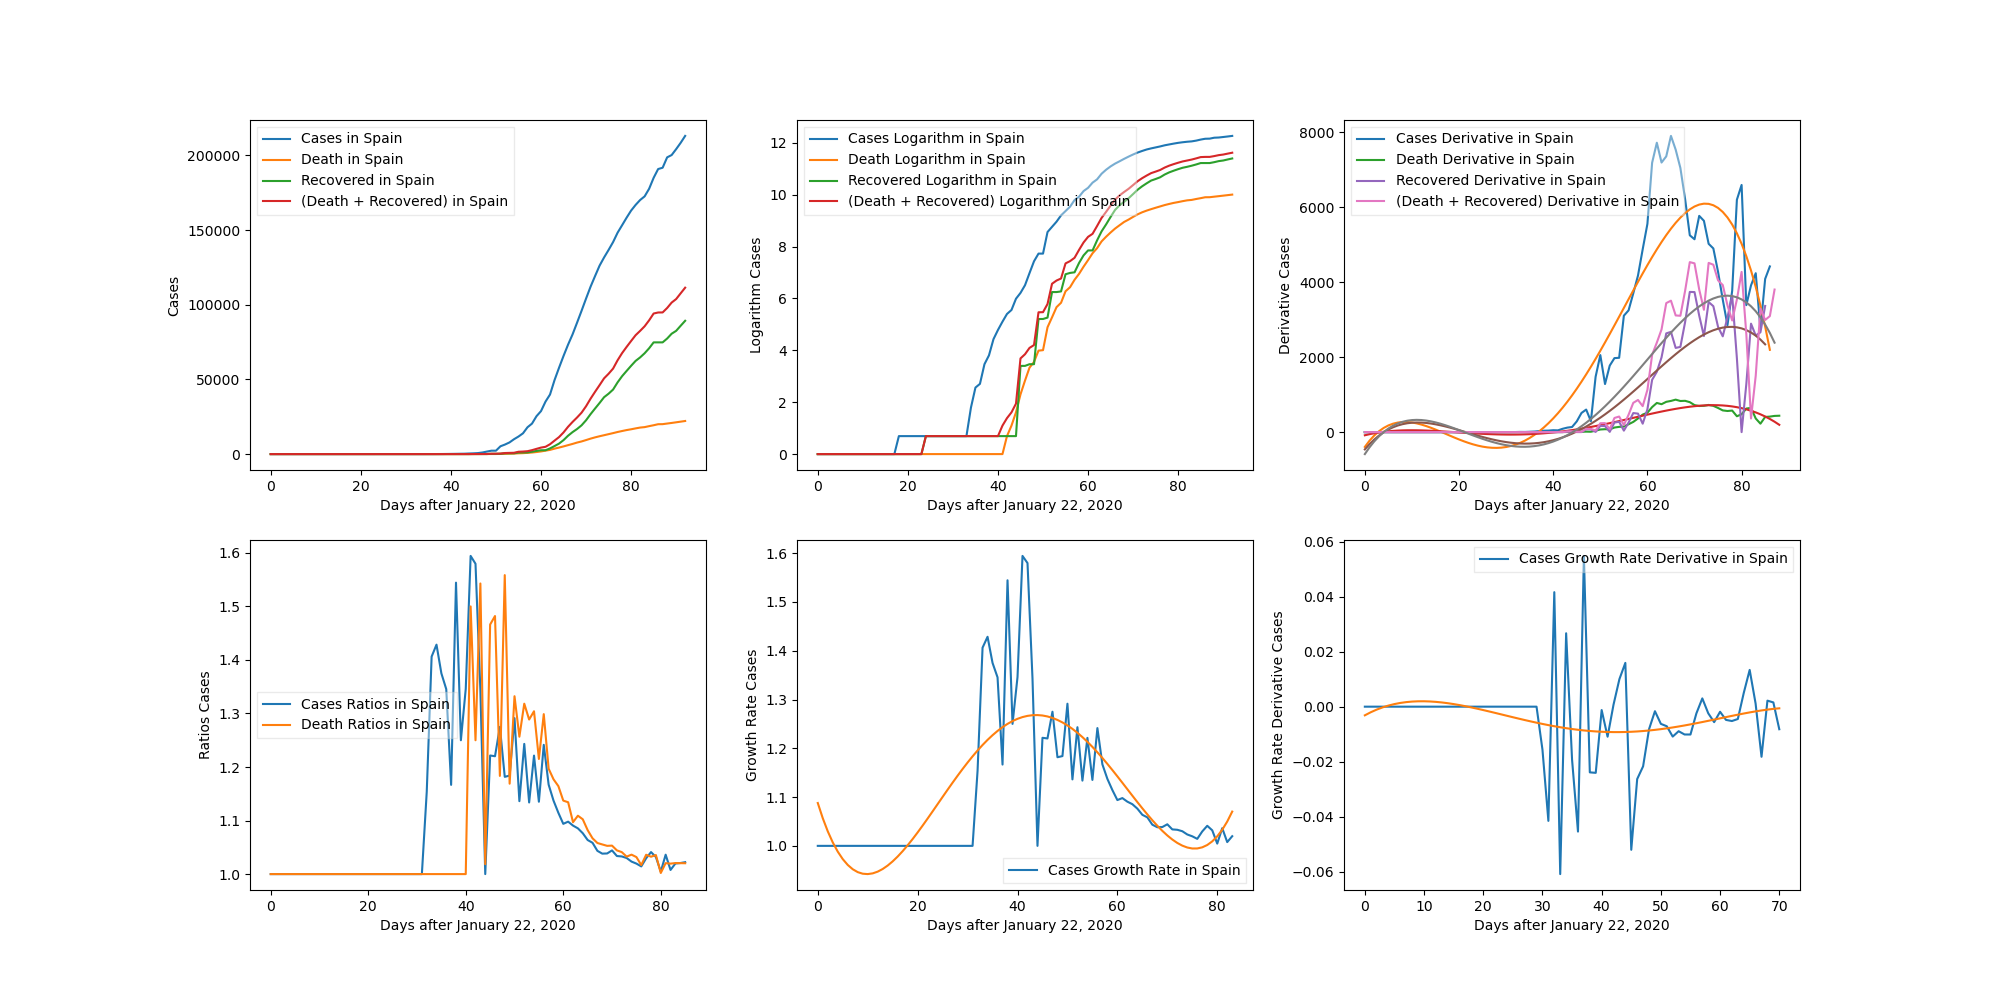
\includegraphics[width=\textwidth]{plots/spain/analyze.png}
                \end{center}
                The time shift of Spain is similar to that of the United States, but the behavior of the graphs are similar to Italy. This shows that the difference between United States and Italy or Spain was not due to the ten day difference, but in the action against coronavirus.
            \subsubsection{India}
                \begin{center}
                    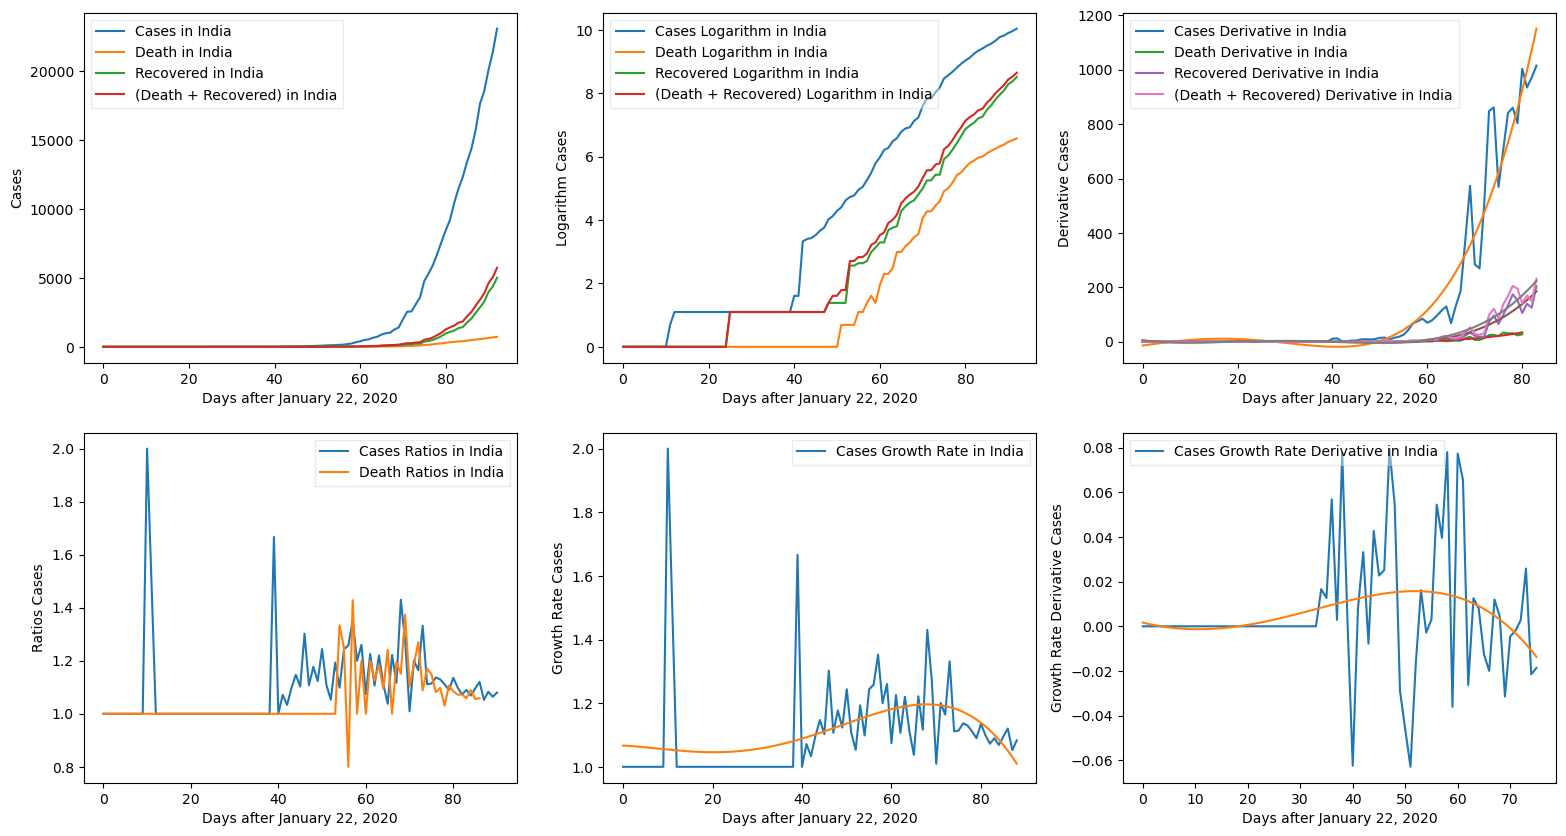
\includegraphics[width=\textwidth]{plots/india/analyze.png}
                \end{center}
                While India's graph of the cases may look similar to the graphs of the other countries, they are very different. This shows the importance of looking at these different transforms of the data (log, derivative, growth rate, ratios, etc.).
                \newline\indent
                India's data is a prime example for exponential growth, which can be seen by taking a look at their logarithmic graph. This graph is almost perfectly linear, with only a slight curve at the very end. India's time shift is similar to that of the United States and Spain, so that it not the reason for them still being in the exponential portion of the logarithmic curve. India's action against the virus is not working to flatten the curve. Looking at the graph of the derivative, we see that it is proportional to the graph of the cases, as expected for exponential growth. 
                \newline\indent
                The growth ratio of India is staying approximately constant at around $1.15$. In a similar manner, the growth rate is not going down. The polyfit curve for $dG^{India}_i/di$ is the opposite of that of the other countries. While this curve does not model $dG^{India}_i/di$ that well, the fact that it is mostly postive indicated that the growth rate is not decreasing enough.
            \subsubsection{France}
                \begin{center}
                    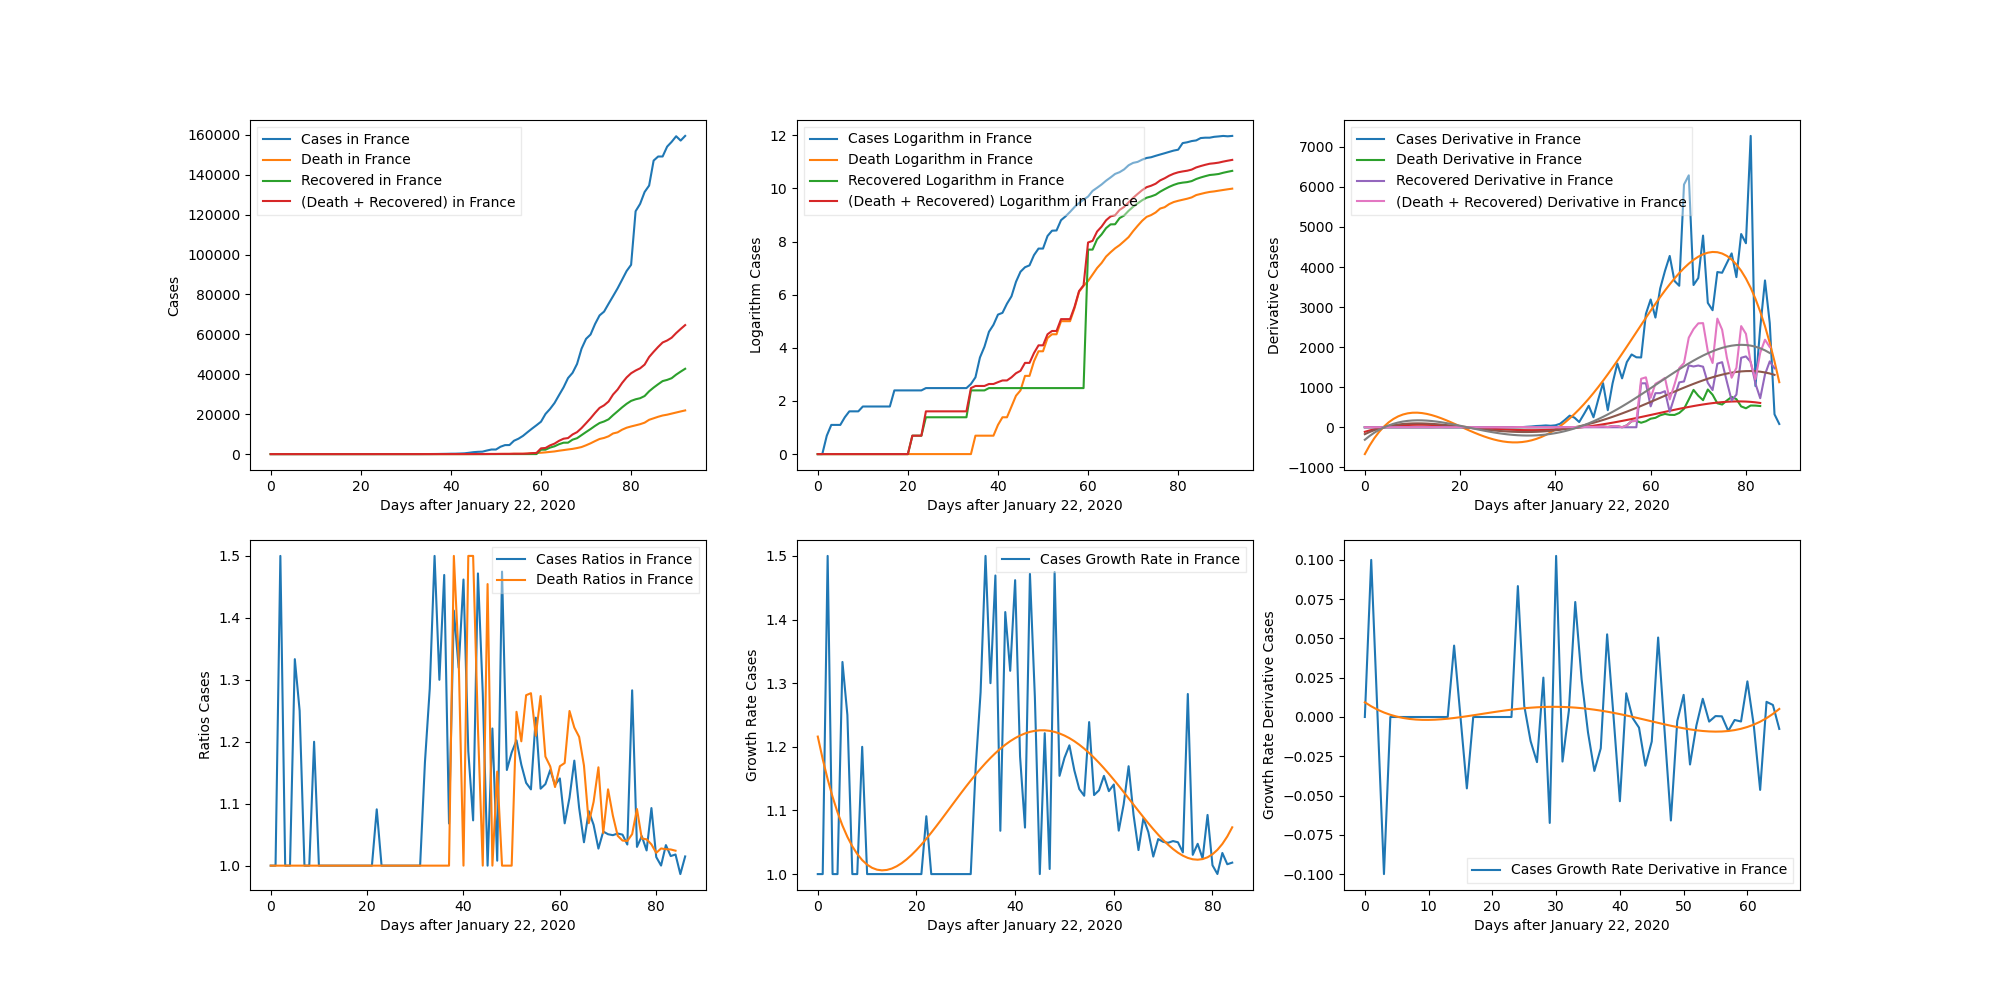
\includegraphics[width=\textwidth]{plots/france/analyze.png}
                \end{center}
                The data for France is very similar to that of the United States. France is time-shifted forward by about 10 less that the United States, making their graphs seem a bit better, but in this case it is very similar to the patterns of the United States.
            \subsubsection{Comparing Amplitudes}
                Most of the analysis I have done up to this point has been about looking at trends in the data but now I will take a look at the amplitudes by estimating the number of cases around $i = 80$ by the graphs for each country.
                \begin{center}
                    \textbf{Amplitudes}
                    \begin{tabular}{||c | c||}
                        \hline
                        Region & Amplitude \\
                        \hline\hline
                        Global & 2.5e6 \\
                        United States & 800,000 \\
                        Spain & 200,000 \\
                        Italy & 175,000 \\
                        France & 160,000 \\
                        China & 80,000 \\
                        India & 20,000 \\
                        \hline
                    \end{tabular}
                \end{center}
                where I have sorted it from greatest to least. By amplitudes it seems that India is doing very well, but from our earlier analysis we know that this may not be true. It is important to take into account both of these factors before making a conclusion.
                \newline\indent
                Another thing to consider while looking at amplitudes is the validity of them. Some countries may not report all of their cases, or they may not even know about them. For this reason, more developed countries and countries with a greater involvement with international health organizations will have larger numbers due to better recording of data. However, if we assume that the ratio of cases reported to true cases stays approximately constant as time passes, we can still look at the trends since we are ignoring amplitudes anyways.
        \subsection{Auto Analysis}
        \label{sec:auto}
            This section will be apply using python to analyze the graphs we have created and use the data to find some intrinsic values and make predictions. These methods will work for any valid value of $X$, but I am going to mainly use the global data. 
            \subsubsection{Finding the Parameters for a Differential Equation}
                The first thing I will do is assume the form of the growth to be logistic. This mean it will follow the differential equation
                \begin{equation}
                    \dfrac{dN^X_i}{di} = c\big(1 - \dfrac{N^X_i}{N^X}\big)N^X_i
                \end{equation}
                Just as a reminder, $N^X$ is the final number of cases in region $X$, or the "carrying capacity" of the spread. Also,
                $$(N^X_i) \rightarrow N^X$$
                \indent
                The first step is to split the data into two sections: one where $N^X_i << N^X$ and the rest. Or mathematically,
                \begin{equation}
                    (N^X_i)_1 = \{N^X_i \in (N^X_i): N^X_i << N^X\} \qquad (N^X_i)_2 = (N^X_i) \backslash (N^X_i)_1
                \end{equation}
                The reason for this splitting is that in $(N^X_i)$, we can ignore the factor $(1 - N^X_i/N^X)$ since $N^X_i << N^X$ implies $N^X_i / N^X << 1$ so $(1 - N^X_i/N^X) \approx 1$. This makes our derivative 
                $$\dfrac{dN^X_i}{di} \approx cN^X_i \qquad N^X_i \in (N^X_i)_1$$
                approximately follows the differential equaiton for exponential growth in $(N^X_i)_1$. Now, there is only one parameter left in this model for the derivative. In theory, I could use gradient descent to find it, but a much simplier way is to just solve for it $\forall N^X_i \in (N^X_i)_1$ and average the results:
                $$c \approx \dfrac{dN^X_i/di}{N^X_i}$$
                Now, taking the average, I set $c$ to 
                \begin{equation}
                    c = \dfrac{1}{m}\sum_{N^X_i \in (N^X_i)_1}\dfrac{dN^X_i/di}{N^X_i}
                \end{equation}
                where $m$ is the length of $(N^X_i)_1$.
                \newline\indent
                Now moving to $\big(\dfrac{dN^X_i/di}{N^X_i}\big)_2$, where we have a logistic growth model again, but now we have $c$ and only need to solve for $N^X$ and then apply the same technique as we did on $c$.
                \newline\indent
                Though some simple algebra
                $$N^X = \big(1 - \dfrac{1}{cN^X_i}\big)^{-1}N^X_i$$
                and taking the mean, I can set
                \begin{equation}
                    N^X = \dfrac{1}{m}\sum_{N^X_i \in (N^X_i)_2}\big(1 - \dfrac{1}{cN^X_i}\big)^{-1}N^X_i
                \end{equation}
                Now both the scaling factor $c$ and the limit/max value $N^X = \lim_{i \rightarrow \infty} N^X_i$ are both known
                \newline
                \textbf{Implementation Details}
                \newline
                To implement this, you must first look at the graphs and choose a place to split your data into the two subsets.
                \begin{center}
                    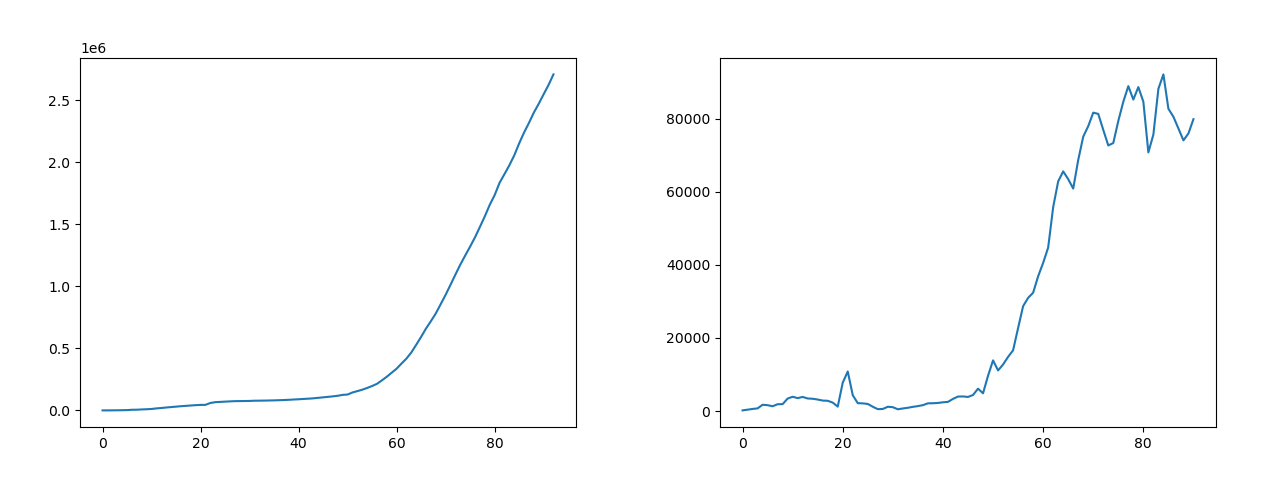
\includegraphics[width=\textwidth]{plots/global/de_parameters/combined.png}
                \end{center}
                Eying out the two graphs ($N^X_i$ and $dN^X_i/di$), I choose to split at $i = 60$. I did this by defining a variable \lstinline{split_point = 60} and then splitting.
                \newline\indent
                A model like this requires a more complete dataset since it is using a pretty basic algorithm to estimate the values for $c$ and $N^X$. Hence, it works pretty will on the China dataset since China's dataset consists of almost the entire logistic curve. However as more data is collected for other countries and as time passes, models like this can be created for other countries as well.
                \newline\indent
                China's output:
                \begin{lstlisting}
                    Finding Differential Equation Parameters - China
                    Enter the split point: 10
                    c: 0.4591556247467866
                    N^X: 83771.24238239802
                \end{lstlisting}
            \subsubsection{Evaluating R-Squared on the Logarithmic Graph}
                Here I will use python to measure how linear the logarithmic of a few countries. The more linear this graph is, the more exponential the number of cases is, implying the action taken against COVID-19 has not been effective.
                \newline\indent
                We can measure how well a linear model fits the logarithmic graph by measure the statistic R-squared, defined by
                \begin{equation}
                    R^2 = \big(\dfrac{||\vec{y} - \hat{y}||}{||\vec{y} - \bar{y}||}\big)^2
                \end{equation}
                where in this case $y$ is the $\ln N^X_i$ and $\hat{y}$ is our linear regression model's prediction from the same input as $\vec{y}$. Also, vector - scalar is defined by elementwise scalar substraction. 
                \newline\indent
                As $R^2$ approaches 1, the fit of the linear model if worse, which is a good thing since that means the curve is flattening out. This is a way to numerically give each country a "rating" on how well they are flattening out the curve.
                \newline\indent
                One important implementation detail is the I only created the linear regression model on the data collected after some growth began. This is to get the best representation of the data's growth rather than including extra data points that have no significance. I did this by only including points with $N^X_i > 10$.                
                \newline
                \begin{center}
                    \textbf{Results}
                    \begin{tabular}{||c | c||}
                        \hline
                        Country & $R^2$ Value \\
                        \hline\hline
                        China & 0.5470569248885822 \\
                        Italy & 0.17500288400296796 \\
                        Spain & 0.14825334735656834 \\
                        Global & 0.08059000856842549 \\
                        France & 0.06241867519925645 \\
                        United States & 0.05848466049484314 \\
                        India & 0.00964424128015847 \\
                        \hline
                    \end{tabular}
                \end{center}
    \section{Modelling}
        \subsection{Problems with Polynomial (Polyfit) Models}
        \label{sec:problems}
            I first considered the idea of a polynomial model back in \hyperref[sec:polys]{Section 2.4}, but as I added more and more data, the number of degrees required kept increasing, which means that a polynomial model will to generalize well to anything outside of the domain it was trained on.
            \newline\indent
            So using \lstinline{np.polyfit} to create an model that will generalize well outside the dataset without just using a large number of degrees\footnote{Using too many degrees is also a problem since the training time will become longer for the same result. We will be losing out on both time and space, the two ways to measure efficiency.} is not possible.
        \subsection{Logistic Growth Model}
            \subsubsection{Solving the Differential Equation}
            \subsubsection{Using Gradient Descent}
            TODO: fix the negative sign and redo entire thing
            \subsubsection{Transforming Features and Linear Regression}
            TODO: Code this (it should be quick)
        \subsection{Transfer Models}
        \subsection{Markov Chain Model}
            TODO: Code Markov Chain Model
        \subsection{RLC Circuit Model}
        \subsection{Neural Network}
            TODO: Code the neural network stuff
    \section{Conclusion}
        \subsection{Country Ranking}
            Spain Italy China France United States Global India
        \subsection{Predictions}
            Not be over before End of May/ Start of June
            \newline
            Max Cases from auto analysis:
    \section{The Code}
        \subsection{Libraries}
        \subsection{Project Structure}
        \subsection{RB Math Package}
            \subsubsection{Gradient Descent and Models}
            \subsubsection{Transforms}
            \subsubsection{Plot Function}
        \subsection{Reading Data}
        \subsection{Plots}
\end{document}